\documentclass{beamer}
\usepackage{graphicx} % Package for images
\usepackage{caption} % Package for numbering figures
\setbeamertemplate{caption}[numbered] % Enable numbering for figures
\captionsetup{font=tiny} % Reduce caption size
\usepackage{tikz}
\usepackage{pgfplots}
\usepackage{multicol}
\usepackage{amsmath}
\usetikzlibrary{trees, positioning}
% Theme choice
\usetheme{CambridgeUS} 
\pgfplotsset{compat=1.18}
\usepackage{helvet} \renewcommand{\familydefault}{\sfdefault}
\setbeamertemplate{headline}{\leavevmode\hbox{}} 
\setbeamertemplate{footline}{%
    \leavevmode%
    \hbox to \paperwidth{%
        \raisebox{1.2ex}[0pt][0pt]{\hspace{1em}\scriptsize\insertframenumber}%
        \hfill%
    }%
}

% Title and author details
\title{$l_1$-K-SVD}
\author{Presented by Dwaipayan Haldar}
\institute{SR Number: 04-03-01-10-42-25-1-27128 \\ Indian Institute of Science, Bengaluru \\ \phantom{123} \\ Original Paper by Dr. Subhadip Mukherjee, \\ Rupam Basu, and Dr. Chandra Sekhar Seelamantula}
\date{}

\begin{document}

% Title slide
\begin{frame}
 \titlepage
\end{frame}

% Content Slides
\begin{frame}{Content}
    \[
    \begin{array}{l}
        1.\ \text{Why Dictionary?} \\[0.6em]
        2.\ \text{General Algorithm} \\[0.6em]
        3.\ \text{K-SVD} \\[0.6em]
        4.\ \text{l1-KSVD} \\[0.6em]
        5.\ \text{Image Denoising}
    \end{array}
    \]
\end{frame}


\begin{frame}{Content}
    \[
    \left[
    \begin{array}{l}
        \text{Why Dictionary?} \\[0.6em]
        \text{General Algorithm} \\[0.6em]
        \text{K-SVD} \\[0.6em]
        \text{l1-KSVD} \\[0.6em]
        \text{Image Denoising}
    \end{array}
    \right]
    \]
\end{frame}

\begin{frame}{Content}
    \[
    \left[
    \begin{array}{l}
        \text{Why Dictionary?} \\[0.45em]
        \text{General Algorithm} \\[0.45em]
        \text{K-SVD} \\[0.45em]
        \text{l1-KSVD} \\[0.45em]
        \text{Image Denoising}
    \end{array}
    \right]
    =
    \underbrace{
    \left[
    \begin{array}{ccccccccc}
    | &       & | &        & | &        & | &     &    | \\
    | &       & | &        & | &        & | &     &     | \\
    5 & \cdot & 8 & \cdot & 9 & \cdot & 32 & \cdot & 46 \\
    | &       & | &        & | &        & | &     &   | \\
    | &       & | &        & | &        & | &     &   | \\
    \end{array}
    \right]}_{\text{Slide number}}
    \left[
    \begin{array}{c}
        1 \\
        \vdots \\
        1 \\
        \vdots \\
        1 \\
        \vdots \\
        1 \\
        \vdots \\
        1
    \end{array}
    \right]
    \]
\end{frame}


%Why Dictionary
\begin{frame}{Why Dictionary?}
    \vspace{0.001cm}
    {\huge
    \[
    y = {\color{red}A}x \phantom{1} \text{s.t.} \phantom{1} \|x\|_0 \leq T_0
    \]
    }
    \[
    y \in \mathbb{R}^{m \times 1}, \qquad
    A \in \mathbb{R}^{m \times n}, \qquad
    x \in \mathbb{R}^{n \times 1}
    \]
\end{frame}

\begin{frame}{Why Dictionary?}
    \vspace{0.1cm}
    {\huge
    \[
    y_i = {\color{red}D}x_i \phantom{1} \text{s.t.} \phantom{1} \|x_i\|_0 \leq T_0
    \]
    }
    \[
    y_i \in \mathbb{R}^{m \times 1}, \qquad
    A \in \mathbb{R}^{m \times n}, \qquad
    x_i \in \mathbb{R}^{n \times 1}
    \]
\end{frame}

\begin{frame}{Why Dictionary?}
    \[
    \underbrace{\left[
    \begin{array}{cccc}
    | & | & & | \\
    y_1 & y_2 & \cdots & y_N \\
    | & | & & |
    \end{array}
    \right]}_{Y_{m \times N}}
    =
    D_{m \times n}
    \underbrace{\left[
    \begin{array}{cccc}
    | & | & & | \\
    x_1 & x_2 & \cdots & x_N \\
    | & | & & |
    \end{array}
    \right]}_{X_{n \times N}}
    \]
    \[
    \text{Here, } m \ll n \ll N.
    \]
\end{frame}

%The 2 step algorithm Slide
\begin{frame}{The 2 steps to success}
\begin{itemize}
    \item \textit{Sparse Coding Step:} Finds the coefficients given the
    dictionary. Use the algorithms we learned in the class.
    \item \textit{Dictionary Update Step:} The dictionary is updated assuming known and fixed coefficients. 
\end{itemize}
\end{frame}

\begin{frame}
\vfill
\centering{\Huge K-SVD}\vfill
\end{frame}


%K-SVD
\begin{frame}{K-SVD - Basic Formulation}
    \[
    \min_{D,X} \left\| Y - DX \right\|_F^2
    \qquad
    \text{subject to}
    \qquad
    \|x_i\|_0 \leq T_0,
    \quad \forall i
    \]
    \[
    \text{where} \left\| \cdot \right\|_F = \sqrt{\sum_{ij}A_{ij}^2}
    \]
\end{frame}

\begin{frame}{K-SVD - Sparse Coding Step}
    Fix the D, then the penalty term can be written as
    \[
    \left\|Y - DX \right\|_F^2 = \sum_{i=1}^{N}\left\|y_i - Dx_i \right\|_2^2
    \]
    \vspace{1.8cm}
\end{frame}

\begin{frame}{K-SVD - Sparse Coding Step}
    Fix the D, then the penalty term can be written as
    \[
    \left\|Y - DX \right\|_F^2 = \sum_{i=1}^{N}\left\|y_i - Dx_i \right\|_2^2
    \]
    So, the minimization problem becomes
    \[
    \min_{x_i} \left\| y_i - D x_i \right\|_2^2
    \qquad
    \text{subject to}
    \qquad
    \|x_i\|_0 \leq T_0,
    \quad \forall i
    \]
    \vspace{0.7cm}
\end{frame}

\begin{frame}{K-SVD - Sparse Coding Step}
    Fix the D, then the penalty term can be written as
    \[
    \left\|Y - DX \right\|_F^2 = \sum_{i=1}^{N}\left\|y_i - Dx_i \right\|_2^2
    \]
    So, the minimization problem becomes
    \[
    \min_{x_i} \left\| y_i - D x_i \right\|_2^2
    \qquad
    \text{subject to}
    \qquad
    \|x_i\|_0 \leq T_0,
    \quad \forall i
    \]
    It can be solved with respect to each $i$ with the help of any suitable
    algorithm taught in the class like OMP, FOCUSS, BP etc.
\end{frame}

\begin{frame}{Detour - The matrix multiplication trivia}
    \[
    DX=
    \left[
    \begin{array}{cccc}
    \begin{array}{c}|\\ d_1\\ |\end{array} &
    \begin{array}{c}|\\ d_2\\ |\end{array} &
    \cdots &
    \begin{array}{c}|\\ d_n\\ |\end{array}
    \end{array}
    \right]_{m\times n}
    \left[
    \begin{array}{c}
    {-}\;x_1\;{-} \\
    {-}\;x_2\;{-} \\
    \vdots \\
    {-}\;x_n\;{-}
    \end{array}
    \right]_{n\times N}
    \]
    \[
    \phantom{\equiv \left[\begin{array}{c}d_1x_1\end{array}\right]_{m\times N}}
    \]
\end{frame}

\begin{frame}{Detour - The matrix multiplication trivia}
    \[
    DX=
    \left[
    \begin{array}{cccc}
    \fcolorbox{red}{white}{$\begin{array}{c}|\\ d_1\\ |\end{array}$} &
    \begin{array}{c}|\\ d_2\\ |\end{array} &
    \cdots &
    \begin{array}{c}|\\ d_n\\ |\end{array}
    \end{array}
    \right]_{m\times n}
    \left[
    \begin{array}{c}
    \fcolorbox{red}{white}{${-}\;x_1\;{-}$} \\
    {-}\;x_2\;{-} \\
    \vdots \\
    {-}\;x_n\;{-}
    \end{array}
    \right]_{n\times N}
    \]
    \[
    \phantom{\equiv \left[\begin{array}{c}d_1x_1\end{array}\right]_{m\times N}}
    \]
\end{frame}

\begin{frame}{Detour - The matrix multiplication trivia}
    \[
    DX=
    \left[
    \begin{array}{cccc}
    \fcolorbox{red}{white}{$\begin{array}{c}|\\ d_1\\ |\end{array}$} &
    \begin{array}{c}|\\ d_2\\ |\end{array} &
    \cdots &
    \begin{array}{c}|\\ d_n\\ |\end{array}
    \end{array}
    \right]_{m\times n}
    \left[
    \begin{array}{c}
    \fcolorbox{red}{white}{${-}\;x_1\;{-}$} \\
    {-}\;x_2\;{-} \\
    \vdots \\
    {-}\;x_n\;{-}
    \end{array}
    \right]_{n\times N}
    \]
    \[
    \equiv
    \left[
    \begin{array}{c}
    d_1x_1
    \end{array}
    \right]_{m\times N}
    \]
\end{frame}

\begin{frame}{Detour - The matrix multiplication trivia}
    \[
    DX=
    \left[
    \begin{array}{cccc}
    \begin{array}{c}|\\ d_1\\ |\end{array} &
    \fcolorbox{red}{white}{$\begin{array}{c}|\\ d_2\\ |\end{array}$} &
    \cdots &
    \begin{array}{c}|\\ d_n\\ |\end{array}
    \end{array}
    \right]_{m\times n}
    \left[
    \begin{array}{c}
    {-}\;x_1\;{-} \\
    \fcolorbox{red}{white}{${-}\;x_2\;{-}$} \\
    \vdots \\
    {-}\;x_n\;{-}
    \end{array}
    \right]_{n\times N}
    \]
    \[
    \equiv
    \left[\begin{array}{c}d_1x_1\end{array}\right]_{m\times N}
    +
    \left[\begin{array}{c}d_2x_2\end{array}\right]_{m\times N}
    \]
\end{frame}

\begin{frame}{Detour - The matrix multiplication trivia}
    \[
    DX=
    \left[
    \begin{array}{cccc}
    \begin{array}{c}|\\ d_1\\ |\end{array} &
    \begin{array}{c}|\\ d_2\\ |\end{array} &
    \cdots &
    \fcolorbox{red}{white}{$\begin{array}{c}|\\ d_n\\ |\end{array}$}
    \end{array}
    \right]_{m\times n}
    \left[
    \begin{array}{c}
    {-}\;x_1\;{-} \\
    {-}\;x_2\;{-} \\
    \vdots \\
    \fcolorbox{red}{white}{${-}\;x_n\;{-}$}
    \end{array}
    \right]_{n\times N}
    \]
    \[
    \equiv
    \left[\begin{array}{c}d_1x_1\end{array}\right]_{m\times N}
    +
    \left[\begin{array}{c}d_2x_2\end{array}\right]_{m\times N}
    + \cdots +
    \left[\begin{array}{c}d_nx_n\end{array}\right]_{m\times N}
    \]
\end{frame}

\begin{frame}{Back to K-SVD}
Now, we know the $X$ matrix obtained by doing the sparse coding step.
We need to update the $D$. That we will do column by column.
So, the penalty term can be written as
\[
\left\|Y-DX\right\|_F^2
=
\left\|
\left(
Y-\sum_{j\neq k} d_jx_j
\right)-d_kx_k
\right\|_F^2
\]
\end{frame}

\begin{frame}{K-SVD - Dictionary Update Step}
Now, we know the $X$ matrix obtained by doing the sparse coding step.
We need to update the $D$. That we will do column by column.
So, the penalty term can be written as
\[
\left\|Y-DX\right\|_F^2
=
\left\|
\left(
Y-\sum_{j\neq k} d_jx_j
\right)-d_kx_k
\right\|_F^2
=
\left\|E_k-d_kx_k\right\|_F^2
\]
\end{frame}

\begin{frame}{K-SVD - Dictionary Update Step}
Now, we know the $X$ matrix obtained by doing the sparse coding step.
We need to update the $D$. That we will do column by column.
So, the penalty term can be written as
\[
\left\|Y-DX\right\|_F^2
=
\left\|
\left(
Y-\sum_{j\neq k} d_jx_j
\right)-d_kx_k
\right\|_F^2
=
\left\|E_k-d_kx_k\right\|_F^2
\]
Here, $E_k$ stands for the error for all the $N$ examples when the
$k^{\text{th}}$ atom is removed.
\end{frame}

\begin{frame}{K-SVD - Dictionary Update Step}
So, here is the easy solution:
\begin{itemize}
    \item Do SVD of $E_k$, $E_k = U \Delta V^T$.
    \item[] \phantom{Select $d_k$ as the first column of $U$ and $x_k$ as the first column of V multiplied by $\Delta(1,1)$.}
    \item[] \phantom{That effectively would give the closest rank 1 approximation via Eckart–Young–Mirsky Theorem (Appendix).}
\end{itemize}

\phantom{\textcolor{red}{Are we done?}}
\end{frame}

\begin{frame}{K-SVD - Dictionary Update Step}
So, here is the easy solution:
\begin{itemize}
    \item Do SVD of $E_k$, $E_k = U \Delta V^T$.
    \item Select $d_k$ as the first column of $U$ and $x_k$ as the first column of V multiplied by $\Delta(1,1)$.
    \item That effectively would give the closest rank 1 approximation via Eckart–Young–Mirsky Theorem (Appendix).
\end{itemize}

\phantom{\textcolor{red}{Are we done?}}
\end{frame}

\begin{frame}{K-SVD - Dictionary Update Step}
So, here is the easy solution:
\begin{itemize}
    \item Do SVD of $E_k$, $E_k = U \Delta V^T$.
    \item Select $d_k$ as the first column of $U$ and $x_k$ as the first column of V multiplied by $\Delta(1,1)$.
    \item That effectively would give the closest rank 1 approximation via Eckart–Young–Mirsky Theorem (Appendix).
\end{itemize}

\textcolor{red}{Are we done?}
\end{frame}

\begin{frame}{K-SVD - Dictionary Learning Step}
Yes, we missed the sparsity. Here is the real solution. 
\begin{itemize}
    \item Define \( \omega_k = \{ i \mid 1 \leq i \leq n, \; x_k(i) \neq 0 \} \)
    \item[] \phantom{Define \( \Omega_k \) as a matrix of size \( N \times |\omega_k| \)
    with ones on the \( (\omega_k(i), i) \)-th entries and zeros elsewhere.}
    \item[] \mbox{}
    \[
    \phantom{\left\|E_k-d_kx_k\right\|_F^2 \rightarrow
    \left\|E_k\Omega_k-d_kx_k\Omega_k\right\|_F^2 =
    \left\| E_k^R - d_kx_k^R \right\|_F^2}
    \]
    \item[] \phantom{Apply the same SVD thing over this modified optimization problem.}
\end{itemize}
\end{frame}

\begin{frame}{K-SVD - Dictionary Learning Step}
Yes, we missed the sparsity. Here is the real solution. 
\begin{itemize}
    \item Define \( \omega_k = \{ i \mid 1 \leq i \leq n, \; x_k(i) \neq 0 \} \)
    \item Define \( \Omega_k \) as a matrix of size \( N \times |\omega_k| \)
    with ones on the \( (\omega_k(i), i) \)-th entries and zeros elsewhere.
    \item[] \mbox{}
    \[
    \phantom{\left\|E_k-d_kx_k\right\|_F^2 \rightarrow
    \left\|E_k\Omega_k-d_kx_k\Omega_k\right\|_F^2 =
    \left\| E_k^R - d_kx_k^R \right\|_F^2}
    \]
    \item[] \phantom{Apply the same SVD thing over this modified optimization problem.}
\end{itemize}
\end{frame}

\begin{frame}{K-SVD - Dictionary Learning Step}
Yes, we missed the sparsity. Here is the real solution. 
\begin{itemize}
    \item Define \( \omega_k = \{ i \mid 1 \leq i \leq n, \; x_k(i) \neq 0 \} \)
    \item Define \( \Omega_k \) as a matrix of size \( N \times |\omega_k| \) with ones on the \( (\omega_k(i), i) \)-th entries and zeros elsewhere.
    \item Change the minimization problem 
    \[
    \left\|E_k-d_kx_k\right\|_F^2 \rightarrow \left\|E_k\Omega_k-d_kx_k\Omega_k\right\|_F^2 = \left\| E_k^R - d_kx_k^R \right\|_F^2
    \]
    \item Apply the same SVD thing over this modified optimization problem.
\end{itemize}
\end{frame}

\begin{frame}{K-SVD - Dictionary Update Step}
So, here is the final solution:
\begin{itemize}
    \item Do SVD of $E_k^R$, $E_k^R = U \Delta V^T$.
    \item Select $d_k$ as the first column of $U$ and $x_k^R$ as the first column of V multiplied by $\Delta(1,1)$.
    \item That effectively would give the closest rank 1 approximation via Eckart–Young–Mirsky Theorem (Appendix).
\end{itemize}

\textcolor{red}{Yes, we are done}
\end{frame}

\begin{frame}{K-SVD - Remarks}
\begin{itemize}
    \item The columns of D remain normalized after each update.
    \item[] \phantom{The support of all the columns of $X$ stays either same or gets smaller after each update.}
    \item[] \phantom{There is simultaneous update of both the $X$ and $D$ in the dictionary update step. Consider two cases, one without simultaneous update and other with simultaneous update.}
\end{itemize}
\[
\phantom{\hat{X}^{\,\mathrm{wsu}} = \hat{X}, 
\hat{D}^{\,\mathrm{wsu}} = \arg\min_{D} J(D,\hat{X})
\quad
\text{s.t. } \|d_j\|_2 = 1 \text{ for all } j}
\]
\[
\phantom{\hat{D}^{\,\mathrm{su}}, \hat{X}^{\,\mathrm{su}}
=
\arg\min_{D,X} J(D,X)
\quad
\text{s.t. } \|d_j\|_2 = 1 \text{ for all } j,\;
\operatorname{supp}(X) \subseteq \Omega}
\]
\[
\phantom{J(\hat{D}^{\,\mathrm{su}}, \hat{X}^{\,\mathrm{su}}) \leq J(\hat{D}^{\,\mathrm{wsu}}, \hat{X}^{\,\mathrm{wsu}})}
\]
\phantom{Case 1 has lesser search space and Case 2. So case 2 is likely to end up in a lesser minima than case 1.}
\end{frame}

\begin{frame}{K-SVD - Remarks}
\begin{itemize}
    \item The columns of D remain normalized after each update.
    \item The support of all the columns of $X$ stays either same or gets smaller after each update.
    \item[] \phantom{There is simultaneous update of both the $X$ and $D$ in the dictionary update step. Consider two cases, one without simultaneous update and other with simultaneous update.}
\end{itemize}
\[
\phantom{\hat{X}^{\,\mathrm{wsu}} = \hat{X}, 
\hat{D}^{\,\mathrm{wsu}} = \arg\min_{D} J(D,\hat{X})
\quad
\text{s.t. } \|d_j\|_2 = 1 \text{ for all } j}
\]
\[
\phantom{\hat{D}^{\,\mathrm{su}}, \hat{X}^{\,\mathrm{su}}
=
\arg\min_{D,X} J(D,X)
\quad
\text{s.t. } \|d_j\|_2 = 1 \text{ for all } j,\;
\operatorname{supp}(X) \subseteq \Omega}
\]
\[
\phantom{J(\hat{D}^{\,\mathrm{su}}, \hat{X}^{\,\mathrm{su}}) \leq J(\hat{D}^{\,\mathrm{wsu}}, \hat{X}^{\,\mathrm{wsu}})}
\]
\phantom{Case 1 has lesser search space and Case 2. So case 2 is likely to end up in a lesser minima than case 1.}
\end{frame}

\begin{frame}{K-SVD - Remarks}
\begin{itemize}
    \item The columns of D remain normalized after each update.
    \item The support of all the columns of $X$ stays either same or gets smaller after each update.
    \item There is simultaneous update of both the $X$ and $D$ in the dictionary update step. Consider two cases, one without simultaneous update and other with simultaneous update.
\end{itemize}
\[
\phantom{\hat{X}^{\,\mathrm{wsu}} = \hat{X}, 
\hat{D}^{\,\mathrm{wsu}} = \arg\min_{D} J(D,\hat{X})
\quad
\text{s.t. } \|d_j\|_2 = 1 \text{ for all } j}
\]
\[
\phantom{\hat{D}^{\,\mathrm{su}}, \hat{X}^{\,\mathrm{su}}
=
\arg\min_{D,X} J(D,X)
\quad
\text{s.t. } \|d_j\|_2 = 1 \text{ for all } j,\;
\operatorname{supp}(X) \subseteq \Omega}
\]
\[
\phantom{J(\hat{D}^{\,\mathrm{su}}, \hat{X}^{\,\mathrm{su}}) \leq J(\hat{D}^{\,\mathrm{wsu}}, \hat{X}^{\,\mathrm{wsu}})}
\]
\phantom{Case 1 has lesser search space and Case 2. So case 2 is likely to end up in a lesser minima than case 1.}
\end{frame}

\begin{frame}{K-SVD - Remarks}
\begin{itemize}
    \item The columns of D remain normalized after each update.
    \item The support of all the columns of $X$ stays either same or gets smaller after each update.
    \item There is simultaneous update of both the $X$ and $D$ in the dictionary update step. Consider two cases, one without simultaneous update and other with simultaneous update.
\end{itemize}
\[
\hat{X}^{\,\mathrm{wsu}} = \hat{X}, 
\hat{D}^{\,\mathrm{wsu}} = \arg\min_{D} J(D,\hat{X})
\quad
\text{s.t. } \|d_j\|_2 = 1 \text{ for all } j
\tag{1}
\]
\[
\hat{D}^{\,\mathrm{su}}, \hat{X}^{\,\mathrm{su}}
=
\arg\min_{D,X} J(D,X)
\quad
\text{s.t. } \|d_j\|_2 = 1 \text{ for all } j,\;
\operatorname{supp}(X) \subseteq \Omega
\tag{2}
\]
\[
J(\hat{D}^{\,\mathrm{su}}, \hat{X}^{\,\mathrm{su}}) \leq J(\hat{D}^{\,\mathrm{wsu}}, \hat{X}^{\,\mathrm{wsu}})
\]
Case 1 has lesser search space and Case 2. So case 2 is likely to end up in a lesser minima than case 1.
\end{frame}

\begin{frame}
\vfill
\centering{\Huge $l_1$-K-SVD}\vfill
\end{frame}

\begin{frame}{$l_1$-K-SVD - Basic Formulation}
    \[
    \min_{D,x_i} \sum_{i=1}^{N}\|y_i-Dx_i\|_1
    + \sum_{i=1}^{N}\lambda_i \|x_i\|_1
    \qquad
    \text{s.t. } \|d_j\|_2 = 1 \text{ for all } j
    \]
\end{frame}

\begin{frame}{$l_1$-K-SVD - Sparse Coding Step}
    \[
    \min_{x_i} \left\|y_i-\hat{D}x_i\right\|_1 + \lambda_i \|x_i\|_1
    \]
\[
\phantom{x_i^{(k+1)}=
\left(\hat{D}^{T}W_{1i}^{(k)}\hat{D}+\lambda_i W_{2i}^{(k)}\right)^{-1}
\hat{D}^{T}W_{1i}^{(k)}y_i}
\]
\[
\phantom{W_{1i}^{(k+1)}(j)=\frac{1}{\left|(y_i-\hat{D}x_i^{(k)})_j\right|+\epsilon},
\qquad
W_{2i}^{(k+1)}(j)=\frac{1}{\left|(x_i^{(k)})_j\right|+\epsilon}}
\]
\end{frame}

\begin{frame}{$l_1$-K-SVD - Sparse Coding Step}
    \[
    \min_{x_i} \left\|y_i-\hat{D}x_i\right\|_1 + \lambda_i \|x_i\|_1
    \]
    The update of $x_i$ in the $k^{th}$ iteration is given as:
    \[
    x_i^{(k+1)}=
    \left(\hat{D}^{T}W_{1i}^{(k)}\hat{D}+\lambda_i W_{2i}^{(k)}\right)^{-1}
    \hat{D}^{T}W_{1i}^{(k)}y_i
    \]
\[
\phantom{W_{1i}^{(k+1)}(j)=\frac{1}{\left|(y_i-\hat{D}x_i^{(k)})_j\right|+\epsilon},
\qquad
W_{2i}^{(k+1)}(j)=\frac{1}{\left|(x_i^{(k)})_j\right|+\epsilon}}
\]
\end{frame}

\begin{frame}{$l_1$-K-SVD - Sparse Coding Step}
    \[
    \min_{x_i} \left\|y_i-\hat{D}x_i\right\|_1 + \lambda_i \|x_i\|_1
    \]
    The update of $x_i$ in the $k^{th}$ iteration is given as:
    \[
    x_i^{(k+1)}=
    \left(\hat{D}^{T}W_{1i}^{(k)}\hat{D}+\lambda_i W_{2i}^{(k)}\right)^{-1}
    \hat{D}^{T}W_{1i}^{(k)}y_i
    \]
    $W_{1i}$ and $W_{2i}$ are diagonal weight matrices that are given by
    \[
    W_{1i}^{(k+1)}(j)=\frac{1}{\left|(y_i-\hat{D}x_i^{(k)})_j\right|+\epsilon},
    \qquad
    W_{2i}^{(k+1)}(j)=\frac{1}{\left|(x_i^{(k)})_j\right|+\epsilon}
    \]
\end{frame}

\begin{frame}{$l_1$-K-SVD - Dictionary Update Step}
    \[
    \min_{D,X} \|Y-DX\|_1
    \qquad
    \text{s.t. } \|d_j\|_2 = 1 \text{ for all } j,\;
    \operatorname{supp}(X) \subseteq \Omega
    \]
    \[
    \text{where}
    \left\| \cdot \right\|_1 = \sum_{i=1}^{N} \left\| y_i - Dx_i \right\|_1
    \]
\end{frame}

\begin{frame}{$l_1$-K-SVD - Dictionary Update Step}
    \[
    \min_{d_k,x_k} \|E_k-d_kx_k\|_1
    \qquad
    \text{s.t. } \operatorname{supp}(x_k)=\omega_k,\; \|d_k\|_2=1
    \]
    \phantom{The support can be included in the optimization problem similar to K-SVD with something like this}
    \[
    \phantom{\|E_k\Omega_k-d_kx_k\Omega_k\|_1
    =
    \|E_k^R-d_kx_k^R\|_1}
    \]
    \phantom{Further simplifying the notation we can say the problem statement as where we need to find the value of u and v.}
    \[
    \phantom{\min_{u,v} \|E-uv^T\|_1
    =
    \min_{u,v}\sum_{i=1}^{N}\|e_i-v_iu\|_1
    \qquad
    \text{s.t. } \|u\|_2=1}
    \]
\end{frame}

\begin{frame}{$l_1$-K-SVD - Dictionary Update Step}
    \[
    \min_{d_k,x_k} \|E_k-d_kx_k\|_1
    \qquad
    \text{s.t. } \operatorname{supp}(x_k)=\omega_k,\; \|d_k\|_2=1
    \]
    The support can be included in the optimization problem similar to K-SVD with something like this 
    \[
    \|E_k\Omega_k-d_kx_k\Omega_k\|_1
    =
    \|E_k^R-d_kx_k^R\|_1
    \]
    \phantom{Further simplifying the notation we can say the problem statement as where we need to find the value of u and v.}
    \[
    \phantom{\min_{u,v} \|E-uv^T\|_1
    =
    \min_{u,v}\sum_{i=1}^{N}\|e_i-v_iu\|_1
    \qquad
    \text{s.t. } \|u\|_2=1}
    \]
\end{frame}

\begin{frame}{$l_1$-K-SVD - Dictionary Update Step}
    \[
    \min_{d_k,x_k} \|E_k-d_kx_k\|_1
    \qquad
    \text{s.t. } \operatorname{supp}(x_k)=\omega_k,\; \|d_k\|_2=1
    \]
    The support can be included in the optimization problem similar to K-SVD with something like this 
    \[
    \|E_k\Omega_k-d_kx_k\Omega_k\|_1
    =
    \|E_k^R-d_kx_k^R\|_1
    \]
    Further simplifying the notation we can say the problem statement as where we need to find the value of u and v.
    \[
    \min_{u,v} \|E-uv^T\|_1
    =
    \min_{u,v}\sum_{i=1}^{N}\|e_i-v_iu\|_1
    \qquad
    \text{s.t. } \|u\|_2=1
    \]
\end{frame}

\begin{frame}{$l_1$-K-SVD - Dictionary Update Step}
    That $l_1$ norm can be approximated by reweighted $l_2$ metric 
    \[
    \sum_{i=1}^{N}\|e_i-v_iu\|_1
    \approx
    \sum_{i=1}^{N}(e_i-v_iu)^T W_i (e_i-v_iu)
    \]
    \[
    \phantom{\text{where}
    W_i(j)=\frac{1}{|(e_i-v_iu)_j|+\epsilon}}
    \]
    \phantom{Differentiating with respect to $u$ and setting to zero for a fixed v}
    \[
    \phantom{
    u=
    \left(\sum_{i=1}^{N} v_i^2 W_i\right)^{-1}
    \left(\sum_{i=1}^{N} v_i W_i e_i\right)}
    \]
    \phantom{Similarily for a fixed u,}
    \[
    \phantom{
    v_i=\frac{u^T W_i e_i}{u^T W_i u},
    }
    \]
    \phantom{This is for one iteration. This is done iteratively for 10 iterations.}
\end{frame}

\begin{frame}{$l_1$-K-SVD - Dictionary Update Step}
    That $l_1$ norm can be approximated by reweighted $l_2$ metric 
    \[
    \sum_{i=1}^{N}\|e_i-v_iu\|_1
    \approx
    \sum_{i=1}^{N}(e_i-v_iu)^T W_i (e_i-v_iu)
    \]
    \[
    \text{where}
    W_i(j)=\frac{1}{|(e_i-v_iu)_j|+\epsilon}
    \]
    Differentiating with respect to $u$ and setting to zero for a fixed v
    \[
    \phantom{
    v_i=\frac{u^T W_i e_i}{u^T W_i u},
    }
    \]
    \phantom{This is for one iteration. This is done iteratively for 10 iterations.}
\end{frame}

\begin{frame}{$l_1$-K-SVD - Dictionary Update Step}
    That $l_1$ norm can be approximated by reweighted $l_2$ metric 
    \[
    \sum_{i=1}^{N}\|e_i-v_iu\|_1
    \approx
    \sum_{i=1}^{N}(e_i-v_iu)^T W_i (e_i-v_iu)
    \]
    \[
    \text{where}
    W_i(j)=\frac{1}{|(e_i-v_iu)_j|+\epsilon}
    \]
    Differentiating with respect to $u$ and setting to zero for a fixed v
    \[
    u=
    \left(\sum_{i=1}^{N} v_i^2 W_i\right)^{-1}
    \left(\sum_{i=1}^{N} v_i W_i e_i\right)
    \]
    Similarily for a fixed u, 
    \[
    v_i=\frac{u^T W_i e_i}{u^T W_i u},
    \]
\end{frame}

\begin{frame}{$l_1$-K-SVD - Final Algorithm to find the best u and v}
\scriptsize
\begin{itemize}
    \item Input: Error matrix $E$, number of iterations $J$.
    \item Initialization:
    Set the iteration counter $t=0$, $u^{(t)}=a$, and
    $v^{(t)}=\sigma b$, where $a$ and $b$ are the left and right singular
    vectors corresponding to the largest singular value $\sigma$ of $E$.
    \item Initialize the weight matrices $W_i^{(t)}=I$, for $i=1,2,\ldots,N$.
    \item Iterate the following steps $J$ times:
    Step 1:
    \[
    W_i^{(t+1)}(j)=\frac{1}{|(e_i-v_i^{(t)}u^{(t)})_j|+\epsilon}
    \]
    Step 2:
    \[
    u^{(t+1)}=
    \Big(\sum_{i=1}^{N} (v_i^{(t)})^2 W_i^{(t+1)}\Big)^{-1}
    \Big(\sum_{i=1}^{N} v_i^{(t)} W_i^{(t+1)} e_i\Big)
    \]
    Step 3:
    \[
    v_i^{(t+1)}=
    \frac{(u^{(t+1)})^T W_i e_i}
    {(u^{(t+1)})^T W_i (u^{(t+1)})}
    \]
    \item Scaling:
    \[
    d_k=\frac{u^{(t)}}{\|u^{(t)}\|_2},
    \qquad
    x_k^R=\|u^{(t)}\|_2 (v^{(t)})^T
    \]
\end{itemize}
\end{frame}


 
\begin{frame}{$l_1$-K-SVD - Remarks}
\begin{itemize}
    \item \textbf{Pruning step (missing from the main algorithm):}
    After each sparse coding step, any coefficient satisfying
    \[
    |x_i(j)| < T_0 \cdot \|X\|_F
    \]
    is pruned to zero. The paper uses $T_0 = 0.03$.
    \item[] \phantom{\textbf{Computationally expensive step:}
    The dictionary update (Algorithm~1) is the bottleneck:
    $K$ atoms $\times$ $J$ inner IRLS iterations, each an $m\times m$ linear solve.
    $\;\Rightarrow\;\mathcal{O}(K\cdot J\cdot m^3)$ work per outer iteration —
    significantly heavier than the single SVD per atom in K-SVD.}
\end{itemize}
\end{frame}

\begin{frame}{$l_1$-K-SVD - Remarks}
\begin{itemize}
    \item \textbf{Pruning step (missing from the main algorithm):}
    After each sparse coding step, any coefficient satisfying
    \[
    |x_i(j)| < T_0 \cdot \|X\|_F
    \]
    is pruned to zero. The paper uses $T_0 = 0.03$.
    \item \textbf{Computationally expensive step:}
    The dictionary update (Algorithm~1) is the bottleneck:
    $K$ atoms $\times$ $J$ inner IRLS iterations, each an $m\times m$ linear solve.
    $\;\Rightarrow\;\mathcal{O}(K\cdot J\cdot m^3)$ work per outer iteration —
    significantly heavier than the single SVD per atom in K-SVD.
\end{itemize}
\end{frame}

% Results

\begin{frame}{Image Denoising — The Core Idea}
\begin{itemize}
    \item \textbf{Corrupted observation:} $y = Dx + w$, where $w$ is noise
    (Gaussian, Laplacian, or missing pixels).
    \item[] \phantom{\textbf{Learn the dictionary $D$:} Train on patches so that $D$
    captures dominant patterns — edges, textures, colour gradients.}
    \item[] \phantom{\textbf{Sparse coding:} Given $D$ and noisy patch $y$, solve}
    \item[] \mbox{}
\end{itemize}
\[
\phantom{\hat{x} = \arg\min_{x}\; \|y - Dx\|_1 + \lambda\|x\|_1}
\]
\phantom{$\ell_1$ fidelity down-weights outlier pixels.}\\[0.3em]
\phantom{\textbf{Reconstruct:} $\hat{y} = D\hat{x}$ — sparse $\hat{x}$ discards the noise component.}
\end{frame}

\begin{frame}{Image Denoising — The Core Idea}
\begin{itemize}
    \item \textbf{Corrupted observation:} $y = Dx + w$, where $w$ is noise
    (Gaussian, Laplacian, or missing pixels).
    \item \textbf{Learn the dictionary $D$:} Train on patches so that $D$
    captures dominant patterns — edges, textures, colour gradients.
    \item[] \phantom{\textbf{Sparse coding:} Given $D$ and noisy patch $y$, solve}
    \item[] \mbox{}
\end{itemize}
\[
\phantom{\hat{x} = \arg\min_{x}\; \|y - Dx\|_1 + \lambda\|x\|_1}
\]
\phantom{$\ell_1$ fidelity down-weights outlier pixels.}\\[0.3em]
\phantom{\textbf{Reconstruct:} $\hat{y} = D\hat{x}$ — sparse $\hat{x}$ discards the noise component.}
\end{frame}

\begin{frame}{Image Denoising — The Core Idea}
\begin{itemize}
    \item \textbf{Corrupted observation:} $y = Dx + w$, where $w$ is noise
    (Gaussian, Laplacian, or missing pixels).
    \item \textbf{Learn the dictionary $D$:} Train on patches so that $D$
    captures dominant patterns — edges, textures, colour gradients.
    \item \textbf{Sparse coding:} Given $D$ and noisy patch $y$, solve
    \item[] \mbox{}
\end{itemize}
\[
\hat{x} = \arg\min_{x}\; \|y - Dx\|_1 + \lambda\|x\|_1
\]
$\ell_1$ fidelity down-weights outlier pixels.\\[0.3em]
\phantom{\textbf{Reconstruct:} $\hat{y} = D\hat{x}$ — sparse $\hat{x}$ discards the noise component.}
\end{frame}

\begin{frame}{Image Denoising — The Core Idea}
\begin{itemize}
    \item \textbf{Corrupted observation:} $y = Dx + w$, where $w$ is noise
    (Gaussian, Laplacian, or missing pixels).
    \item \textbf{Learn the dictionary $D$:} Train on patches so that $D$
    captures dominant patterns — edges, textures, colour gradients.
    \item \textbf{Sparse coding:} Given $D$ and noisy patch $y$, solve
    \item[] \mbox{}
\end{itemize}
\[
\hat{x} = \arg\min_{x}\; \|y - Dx\|_1 + \lambda\|x\|_1
\]
$\ell_1$ fidelity down-weights outlier pixels.\\[0.3em]
\textbf{Reconstruct:} $\hat{y} = D\hat{x}$ — sparse $\hat{x}$ discards the noise component.
\end{frame}


\begin{frame}{Paper Result — Figure 6 (Mukherjee et al.\ 2016)}
\begin{center}
    \includegraphics[width=0.92\textwidth, page=9]{l1-K-SVD.pdf}
\end{center}
\end{frame}

\begin{frame}{Simulation Result A — Gaussian Noise ($\sigma = 20$)}
\begin{figure}
    \centering
    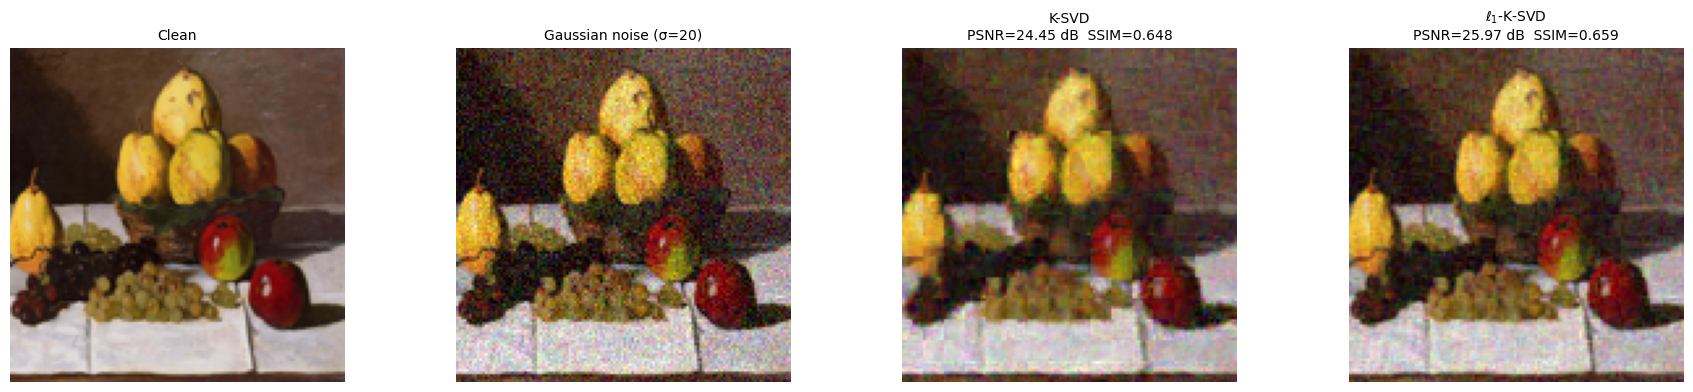
\includegraphics[width=\textwidth]{Output_Images/gaussian_noise.png}
    \caption{4-panel comparison on an impressionist painting.
    Left to right: clean image, noisy input ($\sigma=20/255$),
    K-SVD reconstruction, $\ell_1$-K-SVD reconstruction.
    Both methods perform similarly under Gaussian noise, consistent
    with the $\ell_2$ optimality of K-SVD in this regime.}
\end{figure}
\end{frame}

\begin{frame}{Simulation Result B — Laplacian Noise (same RMS power)}
\begin{figure}
    \centering
    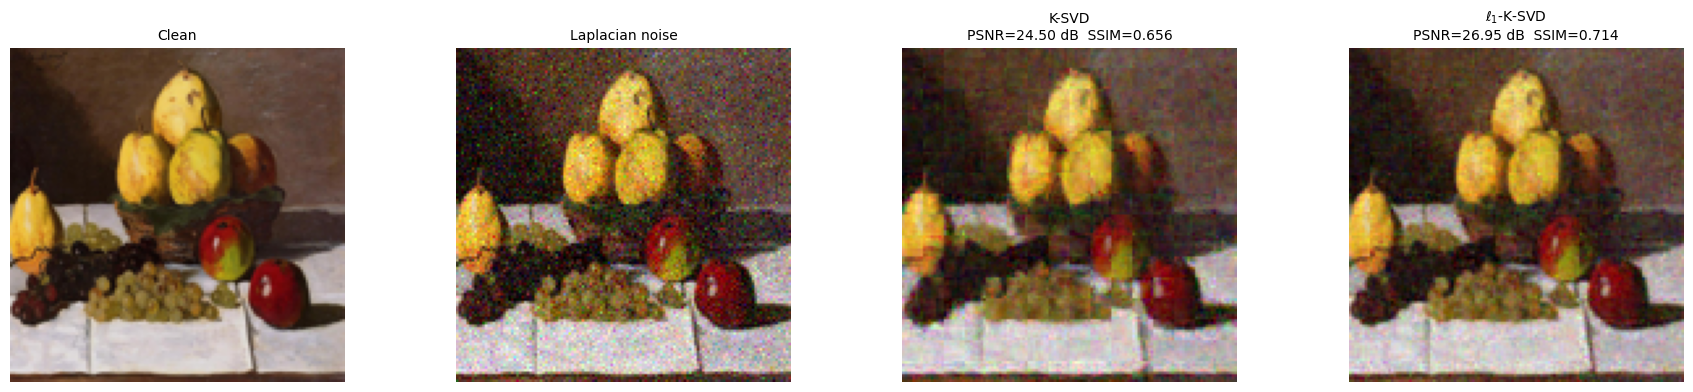
\includegraphics[width=\textwidth]{Output_Images/laplacian_noise.png}
    \caption{Same test image corrupted with Laplacian noise at the same
    RMS power as the Gaussian case.
    $\ell_1$-K-SVD achieves higher PSNR and SSIM because its
    $\ell_1$ data-fidelity term is the natural MAP estimator under a
    Laplacian noise model, while K-SVD's $\ell_2$ criterion is
    sensitive to heavy tails.}
\end{figure}
\end{frame}

\begin{frame}{Simulation Result C — Inpainting (20\% Pixels Removed)}
\begin{figure}
    \centering
    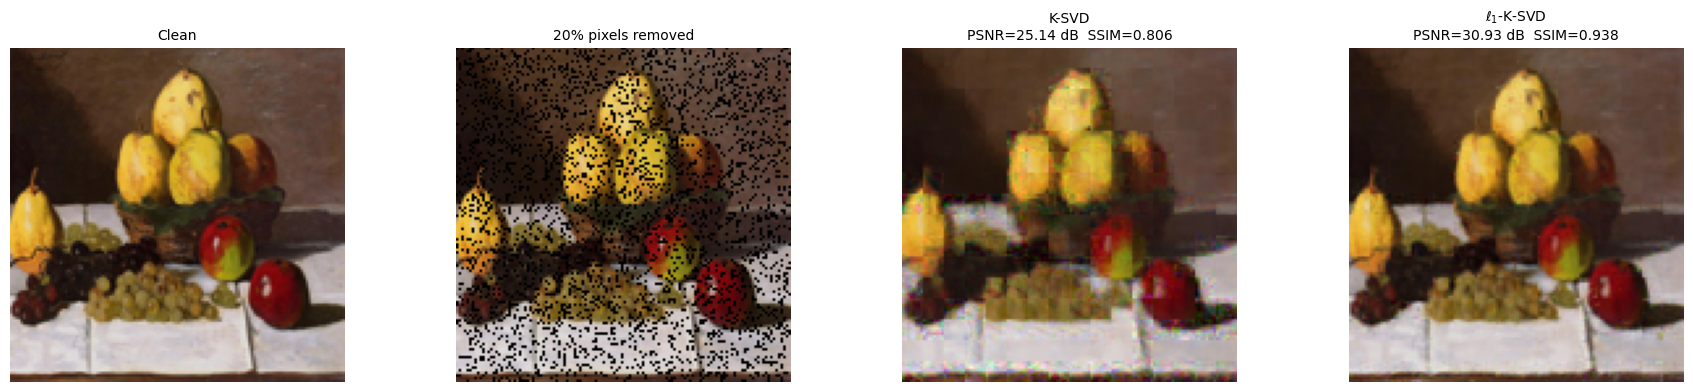
\includegraphics[width=\textwidth]{Output_Images/Removed_pixels.png}
    \caption{20\% of pixels randomly zeroed before reconstruction.
    Missing-data-aware sparse coding (fitting only over observed entries)
    allows $\ell_1$-K-SVD to recover fine texture and colour with
    noticeably higher SSIM than K-SVD.}
\end{figure}
\end{frame}


%  APPENDIX

\appendix

\begin{frame}
\vfill
\centering{\Huge Appendix}\vfill
\end{frame}

% Appendix A: Proof of ℓ₁ Sparse Coding

\begin{frame}{Appendix A: Proof of $\ell_1$ Sparse Coding Step}
\textbf{Problem:}
\[
\min_x \;\|y - Dx\|_1 + \lambda\|x\|_1
\]
Let $r_j = (y-Dx)_j$. Objective $=\displaystyle\sum_j|r_j|+\lambda\sum_i|x_i|$
\[
\phantom{|z|\approx\frac{z^2}{|z^{(k)}|+\epsilon}}
\]
\phantom{IRLS approximation: replace each $|\cdot|$ by a weighted square.}\\[0.3em]
\phantom{Define diagonal weight matrices $W_1^{(k)}$ and $W_2^{(k)}$.}
\end{frame}

\begin{frame}{Appendix A: Proof of $\ell_1$ Sparse Coding Step}
\textbf{Problem:}
\[
\min_x \;\|y - Dx\|_1 + \lambda\|x\|_1
\]
\textbf{IRLS approximation:}
\[
|z|\approx\frac{z^2}{|z^{(k)}|+\epsilon}
\]
Define diagonal weight matrices:
\[
W_1^{(k)}(j)=\frac{1}{|r_j^{(k)}|+\epsilon},\qquad W_2^{(k)}(i)=\frac{1}{|x_i^{(k)}|+\epsilon}
\]
\phantom{Then $\sum_j|r_j|\approx r^TW_1^{(k)}r$ and $\sum_i|x_i|\approx x^TW_2^{(k)}x$}\\[0.3em]
\phantom{\textbf{Surrogate:} $\min_x\;(y-Dx)^TW_1(y-Dx)+\lambda\,x^TW_2x$}
\end{frame}

\begin{frame}{Appendix A: Proof of $\ell_1$ Sparse Coding Step}
\textbf{IRLS weights:}
\[
W_1^{(k)}(j)=\frac{1}{|r_j^{(k)}|+\epsilon},\qquad W_2^{(k)}(i)=\frac{1}{|x_i^{(k)}|+\epsilon}
\]
So $\sum_j|r_j|\approx r^TW_1r$ and $\sum_i|x_i|\approx x^TW_2x$.
\textbf{Surrogate quadratic:}
\[
\min_x\;(y-Dx)^TW_1(y-Dx)+\lambda\,x^TW_2x
\]
\textbf{Expand:}
\[
=\;x^T\!\left(D^TW_1D+\lambda W_2\right)x - 2x^TD^TW_1y + \text{const}
\]
\phantom{Set gradient to zero $\Rightarrow$ normal equations.}
\end{frame}

\begin{frame}{Appendix A: Proof of $\ell_1$ Sparse Coding Step}
\textbf{Normal equations} (set gradient to zero):
\[
\left(D^TW_1^{(k)}D+\lambda W_2^{(k)}\right)x = D^TW_1^{(k)}y
\]
\textbf{Closed-form update:}
\[
\boxed{x^{(k+1)}=\left(D^TW_1^{(k)}D+\lambda W_2^{(k)}\right)^{-1}D^TW_1^{(k)}y}
\]
\textbf{Weight updates} (from definitions):
\[
W_1^{(k+1)}(j)=\frac{1}{\left|(y-Dx^{(k)})_j\right|+\epsilon},\qquad
W_2^{(k+1)}(i)=\frac{1}{\left|x_i^{(k)}\right|+\epsilon}
\]
\end{frame}

% Appendix B: Motivation for the ℓ₁ Objective (Section 2.1) 

\begin{frame}{Appendix B: Motivation for the $\ell_1$ Objective}
\textbf{Bayesian setup.} Assume observations follow $y_n = Dx_n + w_n$.\\[0.5em]
\textbf{Laplacian noise model:}
\[
p(\mathbf{w}_n)=\prod_{j=1}^{m}\frac{1}{2\gamma_n}\exp\!\left(-\frac{|(w_n)_j|}{\gamma_n}\right)
\]
\phantom{\textbf{Laplacian prior on coefficients:}}
\[
\phantom{p(\mathbf{x}_n)=\prod_{j=1}^{K}\frac{1}{2\rho_n}\exp\!\left(-\frac{|(x_n)_j|}{\rho_n}\right)}
\]
\phantom{Laplacian noise motivates $\ell_1$ data fidelity; Laplacian prior motivates $\ell_1$ regularisation.}
\end{frame}

\begin{frame}{Appendix B: Motivation for the $\ell_1$ Objective}
\textbf{Laplacian noise:}
\[
p(\mathbf{w}_n)=\prod_{j=1}^{m}\frac{1}{2\gamma_n}\exp\!\left(-\frac{|(w_n)_j|}{\gamma_n}\right)
\]
\textbf{Laplacian prior on coefficients:}
\[
p(\mathbf{x}_n)=\prod_{j=1}^{K}\frac{1}{2\rho_n}\exp\!\left(-\frac{|(x_n)_j|}{\rho_n}\right)
\]
\phantom{\textbf{MAP estimation:} maximise $\log p(\mathbf{x}_n|\mathbf{y}_n)\propto\log p(\mathbf{y}_n|\mathbf{x}_n)+\log p(\mathbf{x}_n)$}
\[
\phantom{\Rightarrow\;\arg\min_{\mathbf{x}_n}\;\frac{\lambda_n}{\mu_n}\|\mathbf{y}_n-D\mathbf{x}_n\|_1+\|\mathbf{x}_n\|_1}
\]
\end{frame}

\begin{frame}{Appendix B: Motivation for the $\ell_1$ Objective}
\textbf{Laplacian noise:} $p(\mathbf{w}_n)\propto\exp\!\left(-\|\mathbf{w}_n\|_1/\gamma_n\right)$\\[0.3em]
\textbf{Laplacian prior:} $p(\mathbf{x}_n)\propto\exp\!\left(-\|\mathbf{x}_n\|_1/\rho_n\right)$\\[0.5em]
\textbf{MAP estimation:} maximise $\log p(\mathbf{x}_n|\mathbf{y}_n)$
\[
\Rightarrow\;\arg\min_{\mathbf{x}_n}\;\frac{1}{\gamma_n}\|\mathbf{y}_n-D\mathbf{x}_n\|_1+\frac{1}{\rho_n}\|\mathbf{x}_n\|_1
\]
Setting $\lambda_n = \gamma_n/\rho_n$ and summing over all $n$:
\[
\boxed{\min_{D,\,\mathbf{x}_n}\;\sum_{n=1}^{N}\|\mathbf{y}_n-D\mathbf{x}_n\|_1+\lambda_n\|\mathbf{x}_n\|_1}
\]
This is exactly the $\ell_1$-K-SVD objective (Eq.\ 1 in the paper).
\end{frame}

% Appendix C: The ℓp-K-SVD Algorithm

\begin{frame}{Appendix C: The $\ell_p$-K-SVD Algorithm}
\textbf{Generalised objective} ($0<p\leq 1$):
\[
\min_{D,\,\mathbf{x}_n}\;\sum_{n=1}^{N}\|\mathbf{y}_n-D\mathbf{x}_n\|_p^p+\lambda_n\|\mathbf{x}_n\|_p^p
\quad\text{s.t. }\|d_j\|_2=1
\]
\phantom{Corresponds to a \textbf{generalized $p$-Gaussian} distribution:}
\[
\phantom{p_{\mathrm{gen}}(\mathbf{u})\propto\exp\!\left(-\frac{\|\mathbf{u}\|_p^p}{p\,\sigma^p}\right)}
\]
\phantom{For $0<p<1$: even heavier-tailed than Laplacian $\Rightarrow$ sparser solutions.}
\end{frame}

\begin{frame}{Appendix C: The $\ell_p$-K-SVD Algorithm}
\textbf{Generalised objective:}
\[
\min_{D,\,\mathbf{x}_n}\;\sum_{n=1}^{N}\|\mathbf{y}_n-D\mathbf{x}_n\|_p^p+\lambda_n\|\mathbf{x}_n\|_p^p
\]
\textbf{Generalized $p$-Gaussian Bayesian interpretation:}
\[
p_{\mathrm{gen}}(\mathbf{u})\propto\prod_{j}\exp\!\left(-\frac{|u_j|^p}{p\,\sigma_n^p}\right)
\]
MAP maximisation $\Rightarrow$ the $\ell_p^p$ objective above.\\[0.4em]
\phantom{\textbf{Modified IRLS weights} (sparse coding step):}
\[
\phantom{W_{1n}^{(k+1)}(j)=\frac{1}{\left|(\mathbf{y}_n-\hat{D}\mathbf{x}_n^{(k)})_j\right|^{2-p}+\epsilon},
\quad
W_{2n}^{(k+1)}(j)=\frac{1}{\left|(x_n^{(k)})_j\right|^{2-p}+\epsilon}}
\]
\end{frame}

\begin{frame}{Appendix C: The $\ell_p$-K-SVD Algorithm}
\textbf{Modified IRLS weights} (sparse coding, replace $|\cdot|$ with $|\cdot|^{2-p}$):
\[
W_{1n}^{(k+1)}(j)=\frac{1}{\left|(\mathbf{y}_n-\hat{D}\mathbf{x}_n^{(k)})_j\right|^{2-p}+\epsilon},
\quad
W_{2n}^{(k+1)}(j)=\frac{1}{\left|(x_n^{(k)})_j\right|^{2-p}+\epsilon}
\]
\textbf{Modified dictionary update weight} (Algorithm~1, Step~1):
\[
W_n^{(t+1)}(j)=\frac{1}{\left|(\mathbf{e}_n-v_n\mathbf{u}^{(t)})_j\right|^{2-p}+\epsilon}
\]
At $p=1$: recovers $\ell_1$-K-SVD exactly.\\
At $0<p<1$: even sparser solutions, better for impulsive noise.
\end{frame}

% Appendix D: K-SVD as a Generalisation of K-Means 

\begin{frame}{Appendix D: K-SVD as a Generalisation of K-Means}
\textbf{Vector Quantisation (K-means) problem:}
\[
\min_{C,\,X}\;\|Y-CX\|_F^2
\quad\text{s.t. } x_i = e_k \text{ for some } k
\]
$e_k$ is the $k$-th standard basis vector (one-hot). Each signal is represented by \emph{exactly one} codeword column of $C$.\\[0.5em]
\phantom{\textbf{Limitation:} one-hot constraint forces $\|x_i\|_0 = 1$ — a single prototype per signal.}\\[0.3em]
\phantom{Signals with complex structure cannot be well represented.}
\end{frame}

\begin{frame}{Appendix D: K-SVD as a Generalisation of K-Means}
\textbf{K-means:}
\[
\min_{C,\,X}\;\|Y-CX\|_F^2
\quad\text{s.t. } x_i = e_k \;\Rightarrow\; \|x_i\|_0 = 1
\]
\textbf{Limitation:} only one prototype contributes per signal.\\[0.5em]
\textbf{K-SVD generalisation:} relax the one-hot constraint
\[
\min_{D,\,X}\;\|Y-DX\|_F^2
\quad\text{s.t. }\|x_i\|_0\leq T_0,\quad\forall\,i
\]
Allow up to $T_0$ dictionary atoms to contribute — sparse, not binary.\\[0.3em]
\phantom{Both algorithms share the same alternating structure: sparse coding then dictionary update.}
\end{frame}

\begin{frame}{Appendix D: K-SVD as a Generalisation of K-Means}
\textbf{K-means:} $\|x_i\|_0=1$, coefficients are $1$, codeword columns are means.\\[0.3em]
\textbf{K-SVD:} $\|x_i\|_0\leq T_0$, coefficients are real-valued, atoms updated via SVD.\\[0.5em]
\textbf{Same alternating structure:}
\begin{itemize}
    \item \textit{Sparse coding step}: assign signals to atoms (K-means: nearest neighbour; K-SVD: OMP/BP)
    \item \textit{Dictionary update step}: update each atom/codeword given current assignments
\end{itemize}
K-SVD is to K-means as $\ell_0\leq T_0$ is to $\ell_0=1$.
\end{frame}

% Appendix E: Eckart–Young–Mirsky Theorem 

\begin{frame}{Appendix E: Eckart--Young--Mirsky Theorem}
\textbf{Theorem} (Eckart--Young 1936, Mirsky 1960).\\[0.4em]
Let $A\in\mathbb{R}^{m\times n}$ with SVD
\[
A = U\Sigma V^T, \quad \sigma_1\geq\sigma_2\geq\cdots\geq\sigma_p\geq 0,\quad p=\min(m,n).
\]
The rank-$r$ matrix that minimises $\|A-B\|_F$ is
\[
A_r = \sum_{i=1}^{r}\sigma_i\,\mathbf{u}_i\mathbf{v}_i^T
\]
and the minimum error is $\|A-A_r\|_F = \sqrt{\sigma_{r+1}^2+\cdots+\sigma_p^2}$.\\[0.4em]
\phantom{\textbf{Proof idea:} use unitary invariance of $\|\cdot\|_F$ to reduce to the diagonal case.}
\end{frame}

\begin{frame}{Appendix E: Eckart--Young--Mirsky Theorem}
\textbf{Theorem.} $A_r = \sum_{i=1}^{r}\sigma_i\mathbf{u}_i\mathbf{v}_i^T$ minimises $\|A-B\|_F$ over $\mathrm{rank}(B)\leq r$.\\[0.5em]
\textbf{Step 1 — Unitary invariance.}
For any unitary $U,V$: $\|A-B\|_F = \|U^T(A-B)V\|_F$.\\[0.3em]
Writing $A=U\Sigma V^T$:
\[
\|A-B\|_F = \|\Sigma - C\|_F, \qquad C = U^TBV,\quad \mathrm{rank}(C)=\mathrm{rank}(B)\leq r.
\]
\phantom{Reduces the problem: find the best rank-$r$ approximation to the \emph{diagonal} matrix $\Sigma$.}
\end{frame}

\begin{frame}{Appendix E: Eckart--Young--Mirsky Theorem}
\textbf{Step 1.} $\|A-B\|_F = \|\Sigma-C\|_F$ where $C=U^TBV$, $\mathrm{rank}(C)\leq r$.\\[0.5em]
\textbf{Step 2 — Optimise over rank-$r$ matrices $C$.}
\[
\|\Sigma - C\|_F^2 = \sum_{i}(\sigma_i-C_{ii})^2 + \sum_{i\neq j}C_{ij}^2
\]
Off-diagonal terms $C_{ij}^2\geq 0$ only increase the objective.\\
$\Rightarrow$ optimal $C$ is \emph{diagonal}: $C=\mathrm{diag}(c_1,\ldots,c_p)$.\\[0.3em]
\phantom{Among diagonal rank-$r$ matrices: at most $r$ entries $c_i$ are nonzero.}
\[
\phantom{\min_{c:\;\#\{c_i\neq0\}\leq r}\;\sum_i(\sigma_i-c_i)^2}
\]
\end{frame}

\begin{frame}{Appendix E: Eckart--Young--Mirsky Theorem}
\textbf{Step 2.} Optimal $C$ is diagonal: $\|\Sigma-C\|_F^2=\sum_i(\sigma_i-c_i)^2$, $\mathrm{rank}(C)\leq r$.\\[0.4em]
\textbf{Step 3 — Solve the diagonal problem.}\\
At most $r$ of the $c_i$ can be nonzero. For each active $c_i$: set $c_i=\sigma_i$ (contributes $0$). For inactive $c_i=0$: contributes $\sigma_i^2$.\\[0.3em]
To minimise total: activate the $r$ \emph{largest} singular values.
\[
c_i = \sigma_i \text{ for } i\leq r, \quad c_i=0 \text{ for } i>r.
\]
\textbf{Conclusion:}
\[
C^* = \mathrm{diag}(\sigma_1,\ldots,\sigma_r,0,\ldots,0)
\;\Rightarrow\;
B^* = UC^*V^T = A_r
\]
\[
\|A-A_r\|_F = \sqrt{\sigma_{r+1}^2+\cdots+\sigma_p^2} \qquad \square
\]
\end{frame}

\end{document}
